\documentclass{article}

\usepackage{graphicx}
\usepackage{subfig}
\usepackage{float}
\floatstyle{boxed} 
\restylefloat{figure}
\usepackage[pdftex,
            pdfauthor={Tran Ngoc Hieu Nam},
            pdftitle={DSP report},
            pdfsubject={DSP},
            pdfkeywords={DSP},
            pdfproducer={Latex with hyperref, or other system},
            pdfcreator={pdflatex, or other tool}]{hyperref}

\title{Digital Signal Processing Labwork Report }
\author{Tran Ngoc Hieu Nam BI10-124}
\date{2021\\ April}
\begin{document}
\maketitle
\newpage
\textbf{1.Signal}\newline

\begin{figure}[H]

         \centering
         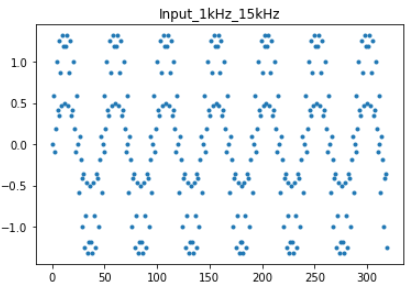
\includegraphics[width=.7\linewidth]{1.1.PNG}
         \caption{plot the signal in time domain}
\end{figure}

\begin{figure}[H]
         		\centering
         		 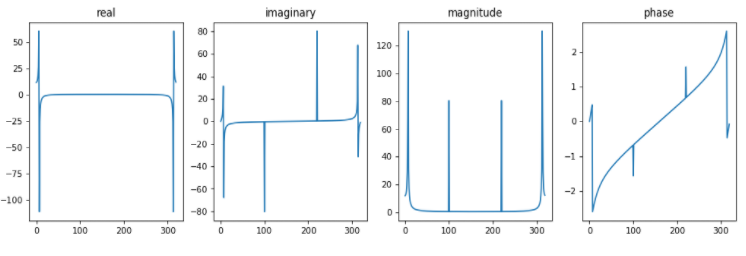
\includegraphics[width=.7\linewidth]{1.2.PNG}
         		\caption{Fast Fourier-transform is used to convert this signal into frequency domain}
\end{figure}

\newpage
\begin{figure}[H]
         \centering
          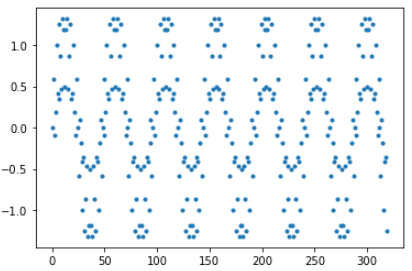
\includegraphics[width=.7\linewidth]{1.3.PNG}
         \caption{using Inverse-FFT to get back to time domain}

\end{figure}

Convert Input\_1kHz\_15kHz signal into frequency domain using fft\newline
Convert Input\_1kHz\_15kHz signal back to time domain using ifft\newline
The figure of this signal in time domain matches the figure of using ifft\newline

\newpage
\textbf{2.System}\newline
\textbf{2.1}
\begin{figure}[H]
         \centering
         \includegraphics[width=.7\linewidth]{2.1.PNG}
         \caption{plot the Impulse response}
 \end{figure}
\textbf{2.2}
\begin{figure}[H]
         \centering
          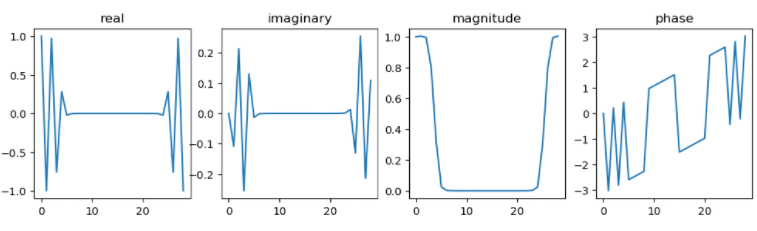
\includegraphics[width=.7\linewidth]{2.2.PNG}
         \caption{convert into frequency, plot real/imaginary/magnitude/phase}
 \end{figure}
\textbf{2.3}
\begin{figure}[H]
         \centering
        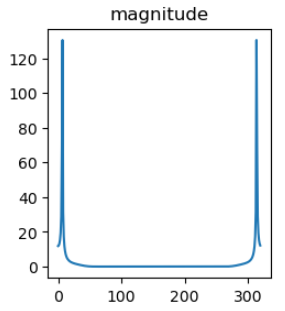
\includegraphics[width=.7\linewidth]{2.3.PNG}
         \caption{calculate the output using time convolution}
\end{figure}

\textbf{2.4}
\begin{figure}[H]
         \centering
          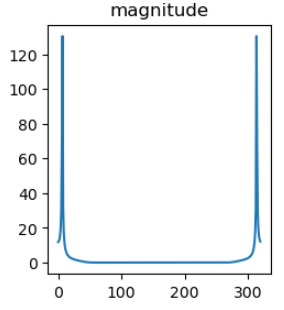
\includegraphics[width=.7\linewidth]{2.4.PNG}
         \caption{frequency multiplication}

\end{figure}
This part is tricky because the impulse response dont have the same shape as the input signal.\newline
The process is that FFT of the output is equal to the multiplication of the 2 components of the convolution:\newline

\textbf{2.5}
Comment: The magnitude of the output by using frequency multiplication and convolution must be the same

\end{document}